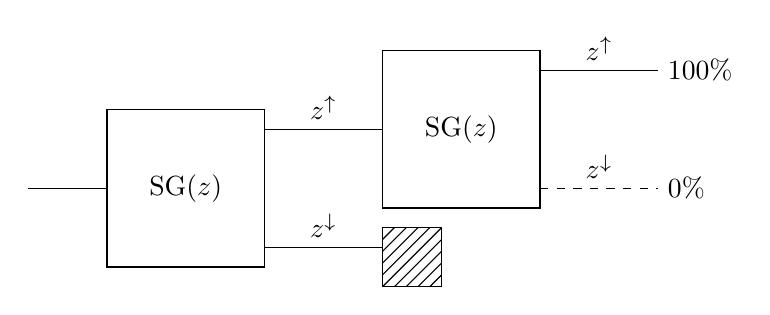
\begin{tikzpicture}[scale=0.5]
    \draw (-2,2) -- (0,2);
    \draw (2,2) node {$\mathrm{SG}(z)$};
    \draw  (0,0) rectangle (4,4);
    \draw (4,3.5) -- (7,3.5) node[above,midway] {$z^\uparrow$};
    \draw (4,0.5) -- (7,0.5) node[above,midway] {$z^\downarrow$};
    \draw  (7,1.5) rectangle (11,5.5);
    \draw  (7,1) rectangle (8.5,-0.5);
    \draw  (11,5) -- (14,5)  node[above,midway] {$z^\uparrow$} node[right] {100\%};
    \draw[dashed]  (11,2) -- (14,2) node[above,midway] {$z^\downarrow$} node[right] {0\%};
    \node at (9,3.5) {$\mathrm{SG}(z)$};
    \foreach \i in {1,...,5} {
    \draw (7+0.3*\i,1)--(7,1-0.3*\i);
    \draw (7+0.3*\i,-0.5)--(8.5,1-0.3*\i);
    };
\end{tikzpicture}
